\documentclass[
	a4paper,
	oneside,
	BCOR = 10mm,
	DIV = 12,
	12pt,
	headings = normal,
]{scrartcl}

%%% Length calculations
\usepackage{calc}
%%%

%%% Support for color
\usepackage{xcolor}
\definecolor{lightblue}{HTML}{03A9F4}
\definecolor{red}{HTML}{F44336}
%%%

%%% Including graphics
\usepackage{graphicx}
%%%

%%% Font selection
\usepackage{fontspec}

\setromanfont{STIX Two Text}[
	SmallCapsFeatures = {LetterSpace = 8},
]

\setsansfont{IBM Plex Sans}[
	Scale = MatchUppercase,
]

\setmonofont{IBM Plex Mono}[
	Scale = MatchUppercase,
]
%%%

%%% Math typesetting
\usepackage{amsmath}

\usepackage{unicode-math}
\setmathfont{STIX Two Math}

\usepackage{IEEEtrantools}
%%%

%%% List settings
\usepackage{enumitem}
\setlist[enumerate]{%
	label*      = {\arabic*.},
	leftmargin  = *,
	labelindent = \parindent,
	topsep      = 1\baselineskip,
	parsep      = 0\baselineskip,
	itemsep     = 1\baselineskip,
	noitemsep, % override itemsep
}

\setlist[itemize]{%
	label*      = {—},
	leftmargin  = *,
	labelindent = \parindent,
	topsep      = 1\baselineskip,
	parsep      = 0\baselineskip,
	itemsep     = 1\baselineskip,
	noitemsep, % override itemsep
}

\setlist[description]{%
	font        = {\rmfamily\upshape\bfseries},
	topsep      = 1\baselineskip,
	parsep      = 0\baselineskip,
	itemsep     = 0\baselineskip,
}

%%%

%%% Structural elements typesetting
\setkomafont{pagenumber}{\rmfamily\upshape}
\setkomafont{disposition}{\rmfamily\bfseries}

% Sectioning
\RedeclareSectionCommand[
	beforeskip = -1\baselineskip,
	afterskip  = 1\baselineskip,
	font       = {\normalsize\bfseries\scshape},
]{section}

\RedeclareSectionCommand[
	beforeskip = -1\baselineskip,
	afterskip  = 1\baselineskip,
	font       = {\normalsize\bfseries\itshape},
]{subsection}

\RedeclareSectionCommand[
	beforeskip = -1\baselineskip,
	afterskip  = 1\baselineskip,
	font       = {\normalsize\bfseries},
]{subsubsection}

\RedeclareSectionCommand[
	beforeskip = -1\baselineskip,
	afterskip  = -0.5em,
	font       = {\normalsize\mdseries\scshape\addfontfeatures{Letters = {UppercaseSmallCaps}}},
]{paragraph}
%%%

%%% Typographic enhancements
\usepackage{microtype}
%%%

%%% Language-specific settings
\usepackage{polyglossia}
\setmainlanguage{ukrainian}
\setotherlanguages{english}
%%%

%%% Captions
\usepackage{caption}
\usepackage{subcaption}

%\DeclareCaptionLabelFormat{closing}{#2)}
%\captionsetup[subtable]{labelformat = closing}

%\captionsetup[subfigure]{labelformat = closing}

\captionsetup[table]{%
	aboveskip = 0\baselineskip,
	belowskip = 0\baselineskip,
}

\captionsetup[figure]{%
	aboveskip = 1\baselineskip,
	belowskip = 0\baselineskip,
}

\captionsetup[subfigure]{%
	labelformat = simple,
	labelformat = brace,
}
%%%

%%% Hyphenated ragged typesetting
\usepackage{ragged2e}
%%%

%%% Table typesetting
\usepackage{booktabs}
\usepackage{longtable}

\usepackage{multirow}

\usepackage{array}
\newcolumntype{v}[1]{>{\RaggedRight\arraybackslash\hspace{0pt}}p{#1}}
\newcolumntype{b}[1]{>{\Centering\arraybackslash\hspace{0pt}}p{#1}}
\newcolumntype{n}[1]{>{\RaggedLeft\arraybackslash\hspace{0pt}}p{#1}}
%%%

%%% Drawing
\usepackage{tikz}
\usepackage{tikzscale}
\usetikzlibrary{positioning}
\usetikzlibrary{arrows.meta} % Stealth arrow tips
\usetikzlibrary{shapes.geometric} % Stealth arrow tips
%%%

%%% SI units typesetting
\usepackage{siunitx}
\sisetup{%
	output-decimal-marker = {,},
	exponent-product      = {\cdot},
	inter-unit-product    = \ensuremath{{} \cdot {}},
	per-mode              = symbol,
}
%%%

%%% Framing code listings
\usepackage{tcolorbox}
\tcbuselibrary{breakable}
\tcbuselibrary{minted}
\tcbuselibrary{skins}

\newtcblisting[
	auto counter, 
	list inside, 
	number within = section,
]{listingpython}[3][]{%
	minted language = python,
	minted style    = bw,
	minted options  = {%
		linenos,
		tabsize = 4,
		breaklines,
		% breakanywhere,
		fontsize = \footnotesize,
		autogobble
	},
	%
	% empty,
	sharp corners,
	colframe         = black,
	colback          = black!0,
	leftrule         = 0em,
	rightrule        = 0em,
	toprule          = 1pt, % orig = 0pt
	bottomrule       = 1pt, % orig = 0pt
	titlerule        = 0.5pt,
	colbacktitle     = black!0,
	coltitle         = black,
	toptitle         = 0.3em,
	bottomtitle      = 0.1em,
	borderline north = {1pt}{0pt}{black},
	borderline south = {1pt}{0pt}{black},
	before skip      = \intextsep,
	after  skip      = \intextsep,
	title            = {Лістинг \thetcbcounter: #2},
	list entry       = {\protect\numberline{\thetcbcounter}#2},
	left = 0em,
	right = 0em,
	%
	listing only,
	breakable,
	%
	label = {#3},
	%
	#1
}

\newtcbinputlisting[auto counter, list inside, number within = section]{\inputpython}[4][]{%
	minted language = python,
	minted style    = bw,
	minted options  = {%
		linenos,
		tabsize = 4,
		breaklines,
		breakbytokenanywhere,
		fontsize = \footnotesize,
	},
	%
	% empty,
	sharp corners,
	colframe         = black,
	colback          = black!0,
	leftrule         = 0em,
	rightrule        = 0em,
	toprule          = 0pt, % orig = 0pt
	bottomrule       = 0pt, % orig = 0pt
	titlerule        = 0.5pt,
	colbacktitle     = black!0,
	coltitle         = black,
	toptitle         = 0.3em,
	bottomtitle      = 0.1em,
	borderline north = {1pt}{0pt}{black},
	borderline south = {1pt}{0pt}{black},
	before skip      = \intextsep,
	after  skip      = \intextsep,
	title            = {Лістинг \thetcbcounter: #3},
	list entry       = {\protect\numberline{\thetcbcounter}#3},
	left = 0em,
	right = 0em,
	%
	listing file={#2},
	listing only,
	breakable,
	%
	label = {#4},
	%
	#1
}

% Customize minted
\usepackage{minted}
\setmintedinline{%
	style = bw,
	breaklines,
}

% Customize minted line numbers
\renewcommand{\theFancyVerbLine}{\ttfamily\scriptsize\arabic{FancyVerbLine}}

%%%

%%% Sideways table
\usepackage{pdflscape}
%%%

%%% Wrap text after sideways table
\usepackage{afterpage}
%%%

%%% Links and hyperreferences
\usepackage{hyperref}
\hypersetup{%
	bookmarksnumbered = true,
	colorlinks      = false,
	linkbordercolor = red,
	urlbordercolor  = lightblue,
	pdfborderstyle  = {/S/U/W 1.5},
}
%%%

%%% Length adjustments
% Set baselineskip, default is 14.5 pt
\linespread{1.068966} % ~15.5 pt
\setlength{\emergencystretch}{1em}
\setlength{\parindent}{1.5em}
\newlength{\gridunitwidth}
\setlength{\gridunitwidth}{\textwidth / 12}
%%%

%%% Custom commands
\newcommand{\allcaps}[1]{{\addfontfeatures{LetterSpace = 8, Kerning = Off}#1}}
\newcommand{\filename}[1]{\texttt{#1}}
\newcommand{\progname}[1]{\texttt{#1}}
\newcommand{\modulename}[1]{\texttt{#1}}
%%%

%%% Custom math commands
\newcommand{\longvar}[1]{\mathit{#1}}
%%%

\begin{document}

\begin{titlepage}
		\begin{center}
			Міністерство освіти і науки України\\
			Національний авіаційний університет\\
			Навчально-науковий інститут комп'ютерних інформаційних технологій\\
			Кафедра комп'ютеризованих систем управління

			\vspace{\fill}
				Лабораторна робота №2\\
				з~дисципліни «Комп'ютерні системи»\\
				на~тему «Моделювання часових характеристик обчислювальних систем та~мереж»\\
				Варіант~№3

			\vspace{\fill}

			\begin{flushright}
				Виконав:\\
				студент \allcaps{ННІКІТ}\\
				групи СП-325\\
				Клокун В.\,Д.\\
				Перевірив:\\
				Ковальов М.\,О.
			\end{flushright}

			Київ 2019
		\end{center}
	\end{titlepage}

	\section{Мета роботи}
		Вивчення методів оцінки трудомісткості алгоритмів.

	\section{Хід роботи}
		Вихідними даними для лабораторної роботи є схема алгоритму~(рис.~\ref{fig:flowchart}). Для побудови матриці переходів за схемою алгоритму також надані значення параметрів, що перевіряються алгоритмом~(табл.~\ref{tab:Xi-Ki-vals}).

		\begin{figure}[!htbp]
			\centering
			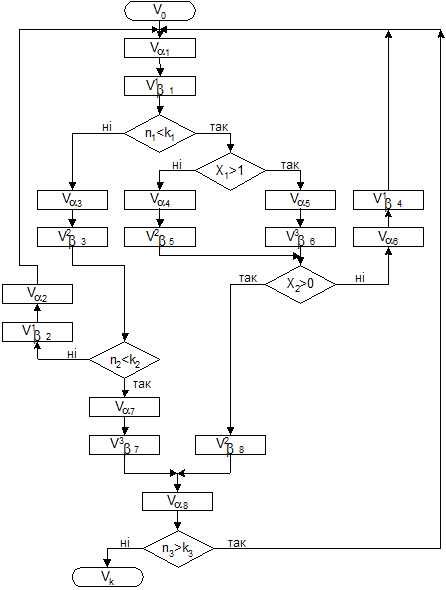
\includegraphics[height = 21\baselineskip]{./assets/y03s02-compsys-lab-02-p01.png}
			\caption{Схема алгоритму}
			\label{fig:flowchart}
		\end{figure}

		\begin{table}[!htbp]
			\newlength{\tmplen}
			\setlength{\tmplen}{9\gridunitwidth / 5}
			\centering
			\caption{Області зміни параметрів~$X_i$, $K_i$, що складають оператор~$V_{\alpha{}i}$}
			\label{tab:Xi-Ki-vals}
			\begin{tabular}{%
				v{3\gridunitwidth - 2\tabcolsep}
				*{5}{n{\tmplen - 2\tabcolsep}}
			}
				\toprule
					Номер варіанта & \multicolumn{5}{r}{Параметр та його значення} \\
					\cmidrule(lr){2-6}
					 & $X_{1}$ & $X_{2}$ & $K_1$ & $K_2$ & $K_3$ \\
				\midrule
					3 & $0, +4$ & $-3, 1$ & 10 & 20 & 30 \\
				\bottomrule
			\end{tabular}
		\end{table}

		\subsection{Обчислення середньої кількості операцій за один прогін алгоритму}
			Нехай~$n_1, \dots, n_{k-1}$~— середня кількість звернень до~операторів~$V_1, \dots, V_{k - 1}$. Тоді середня кількість операцій за один прогін алгоритму~$\theta_{\text{осн}}$ визначається так:
			\begin{IEEEeqnarray}{rCl}
				\label{eq:avg-op-cnt-per-run}
				\theta_{\text{осн}} = \sum_{} n_i \cdot k_i.
			\end{IEEEeqnarray}
			Щоб знайти значення середньої кількості звернень~$n_1, \dots, n_{k-1}$, за~схемою алгоритму визначаємо та~будуємо матрицю ймовірностей переходу, в~якій кожен елемент~$P_{ij}$ визначає ймовірність переходу із стану~$i$ в~стан~$j$~(табл.~\ref{tab:transition-prob}). 

			\afterpage{%
			\begin{landscape}
				\begin{table}
					\centering
					\caption{Матриця ймовірностей переходу схеми алгоритму}
					\label{tab:transition-prob}
					\begin{tabular}{%
						l
						*{17}{r}
					}
						\toprule
							& $V_{\alpha{}1}$ & $V^{1}_{\beta{}1}$ & $V_{\alpha{}2}$ & $V^{1}_{\beta{}2}$ & $V_{\alpha{}3}$ & $V^{2}_{\beta{}3}$ & $V_{\alpha{}4}$ & $V^{1}_{\beta{}4}$ & $V_{\alpha{}5}$ & $V^{2}_{\beta{}5}$ & $V_{\alpha{}6}$ & $V^{3}_{\beta{}6}$ & $V_{\alpha{}7}$ & $V^{3}_{\beta{}7}$ & $V_{\alpha{}8}$ & $V^{2}_{\beta{}8}$ & $V_{k}$ \\ 
						\midrule
							$V_{\alpha{}1}$ &  & \num{1.0} &  &  &  &  &  &  &  &  &  &  &  &  &  &  & \\
							$V^{1}_{\beta{}1}$ &  &  &  &  & \num{0.1} &  & \num{0.225} &  & \num{0.675} &  &  &  &  &  &  &  & \\
							$V_{\alpha{}2}$ & \num{1.0} &  &  &  &  &  &  &  &  &  &  &  &  &  &  &  & \\
							$V^{1}_{\beta{}2}$ &  &  & \num{1.0} &  &  &  &  &  &  &  &  &  &  &  &  &  & \\
							$V_{\alpha{}3}$ &  &  &  &  &  & \num{1.0} &  &  &  &  &  &  &  &  &  &  & \\
							$V^{2}_{\beta{}3}$ &  &  &  & \num{0.05} &  &  &  &  &  &  &  &  & \num{0.95} &  &  &  & \\
							$V_{\alpha{}4}$ &  &  &  &  &  &  &  &  &  & \num{1.0} &  &  &  &  &  &  & \\
							$V^{1}_{\beta{}4}$ & \num{1.0} &  &  &  &  &  &  &  &  &  &  &  &  &  &  &  & \\
							$V_{\alpha{}5}$ &  &  &  &  &  &  &  &  &  &  &  & \num{1.0} &  &  &  &  & \\
							$V^{2}_{\beta{}5}$ &  &  &  &  &  &  &  &  &  &  & \num{0.75} &  &  &  &  & \num{0.25} & \\
							$V_{\alpha{}6}$ &  &  &  &  &  &  &  & \num{1.0} &  &  &  &  &  &  &  &  & \\
							$V^{3}_{\beta{}6}$ &  &  &  &  &  &  &  &  &  &  & \num{0.750} &  &  &  &  & \num{0.25} & \\
							$V_{\alpha{}7}$ &  &  &  &  &  &  &  &  &  &  &  &  &  & \num{1.0} &  &  & \\
							$V^{3}_{\beta{}7}$ & \num{1.0} &  &  &  &  &  &  &  &  &  &  &  &  &  &  &  & \\
							$V_{\alpha{}8}$ & \num{0.03} &  &  &  &  &  &  &  &  &  &  &  &  &  &  &  & \num{0.97}\\
							$V^{2}_{\beta{}8}$ &  &  &  &  &  &  &  &  &  &  &  &  &  &  & \num{1.0} &  & \\
							%
							% $V_{\alpha{}1}$ & & & \num{0.9} & \num{0.025} & \num{0.075}\\
							% $V_{\alpha{}2}$ & \num{1} \\
							% $V_{\alpha{}3}$ & & \num{0.95} & & & & & \num{0.05} \\
							% $V_{\alpha{}4}$ & & & & & & \num{0.75} & & \num{0.25}\\
							% $V_{\alpha{}5}$ & & & & & & \num{0.75} & & \num{0.25}\\
							% $V_{\alpha{}6}$ & \num{1} \\
							% $V_{\alpha{}7}$ & & & & & & & & \num{1} & \\
							% $V_{\alpha{}8}$ & \num{0.03} & & & & & & & & \num{0.97} \\
						\bottomrule
					\end{tabular}
				\end{table}
			\end{landscape}
			}

			За матрицею ймовірностей переходу складаємо систему лінійних алгебраїчних рівнянь:
			% \begin{landscape}
			\begin{IEEEeqnarray}{c}
				% \scriptsize
				\label{eq:sys}
				\left\{ \,
				\begin{IEEEeqnarraybox}[][c]{l}
					\IEEEstrut
						-n_{\alpha{}1} + n_{\alpha{}2} + n_{\beta{}4} + n_{\beta{}7} + \num{+0.030}n_{\alpha{}8} = -1, \\
						n_{\alpha{}1} -n_{\beta{}1} = 0, \\
						-n_{\alpha{}2} + n_{\beta{}2} = 0, \\
						-n_{\beta{}2} + \num{+0.050}n_{\beta{}3} = 0, \\
						\num{+0.100}n_{\beta{}1} -n_{\alpha{}3} = 0, \\
						n_{\alpha{}3} -n_{\beta{}3} = 0, \\
						\num{+0.225}n_{\beta{}1} -n_{\alpha{}4} = 0, \\
						-n_{\beta{}4} + n_{\alpha{}6} = 0, \\
						\num{+0.675}n_{\beta{}1} -n_{\alpha{}5} = 0, \\
						n_{\alpha{}4} -n_{\beta{}5} = 0, \\
						\num{+0.750}n_{\beta{}5} -n_{\alpha{}6} + \num{+0.750}n_{\beta{}6} = 0, \\
						n_{\alpha{}5} -n_{\beta{}6} = 0, \\
						\num{+0.950}n_{\beta{}3} -n_{\alpha{}7} = 0, \\
						n_{\alpha{}7} -n_{\beta{}7} = 0, \\
						-n_{\alpha{}8} + n_{\beta{}8} = 0, \\
						\num{+0.250}n_{\beta{}5} + \num{+0.250}n_{\beta{}6} -n_{\beta{}8} = 0.
					\IEEEstrut
				\end{IEEEeqnarraybox}
				\right.
			\end{IEEEeqnarray}
		%\end{landscape}
			Знаходимо розв'язок системи лінійних алгебраїчних рівнянь і записуємо його. Для операторних вершин:
			\begin{IEEEeqnarray*}{rCl'rCl'rCl'rCl}
				n_{\alpha{}1} &=& \num{4.58}, &% \approx \num{14.73}
				n_{\alpha{}2} &=& \num{0.03}, &% \approx \num{12.59}
				n_{\alpha{}3} &=& \num{0.46}, &% \approx \num{13.25}
				n_{\alpha{}4} &=& \num{1.03}, \\[2\jot] % \approx \num{ 0.39}
				n_{\alpha{}5} &=& \num{3.09}, &% \approx \num{ 1.10}
				n_{\alpha{}6} &=& \num{3.09}, &% \approx \num{ 1.10}
				n_{\alpha{}7} &=& \num{0.44}, &% \approx \num{ 0.66}
				n_{\alpha{}8} &=& \num{1.03}.  % \approx \num{ 1.03}
			\end{IEEEeqnarray*}
			Для файлових вершин:
			\begin{IEEEeqnarray*}{rCl'rCl'rCl'rCl}
				n_{\beta{}1} &=& \num{4.58}, &% \approx \num{14.73}
				n_{\beta{}2} &=& \num{0.02}, &% \approx \num{12.59}
				n_{\beta{}3} &=& \num{0.46}, &% \approx \num{13.25}
				n_{\beta{}4} &=& \num{3.09}, \\[2\jot] % \approx \num{ 0.39}
				n_{\beta{}5} &=& \num{1.03}, &% \approx \num{ 1.10}
				n_{\beta{}6} &=& \num{3.09}, &% \approx \num{ 1.10}
				n_{\beta{}7} &=& \num{0.44}, &% \approx \num{ 0.66}
				n_{\beta{}8} &=& \num{1.03}.  % \approx \num{ 1.03}
			\end{IEEEeqnarray*}
			Отже, розв'язавши систему рівнянь, отримали середні кількості звернень~$n_{1}, \dots, n_{k-1}$ до~операторів~$V_{1}, \dots, V_{k-1}$. 

			Щоб обчислити значення середньої кількості операцій за один прогін алгоритму~$\theta_{\text{осн}}$, необхідно знати значення кількості операцій~$k_i$ кожного оператора~$V_{\alpha{}i}$~(для~заданого варіанту~№3~— табл.~\ref{tab:ki-vals}). 

			\begin{table}[!htbp]
				\centering
				\caption{Число операцій~$k_i$, що складають оператор~$V_{\alpha{}i}$}
				\label{tab:ki-vals}
				\begin{tabular}{%
					v{4\gridunitwidth - 2\tabcolsep}
					*{8}{n{1\gridunitwidth - 2\tabcolsep}}
				}
					\toprule
						Номер варіанта & \multicolumn{8}{r}{Кількість операторів~$V_{\alpha}$} \\
						\cmidrule(lr){2-9}
						 & $V_{\alpha{}_1}$ & $V_{\alpha{}_2}$ & $V_{\alpha{}_3}$ & $V_{\alpha{}_4}$ & $V_{\alpha{}_5}$ & $V_{\alpha{}_6}$ & $V_{\alpha{}_7}$ & $V_{\alpha{}_8}$ \\ 
					\midrule
						3 & 30 & 10 & 30 & 20 & 20 & 30 & 50 & 100\\
					\bottomrule
				\end{tabular}
			\end{table}

			Тепер обчислюємо середню кількість операцій за~один прогін алгоритму. Для цього підставляємо задані значення кількості операцій кожного оператора~(табл.~\ref{tab:ki-vals}) у~формулу~\eqref{eq:avg-op-cnt-per-run}:
			\begin{IEEEeqnarray*}{rCl}
				\theta_{\text{осн}} &=& \sum_{V \in S_o}^{} n_{\alpha{}i} \cdot k_i\\[2\jot]
				                    &=& \num{4.58} \cdot 30 + \num{0.02} \cdot 10 + \num{0.46} \cdot 30 + \num{1.03} \cdot 20 \\
														&&  \>{+} \num{3.09} \cdot 20 + \num{3.09} \cdot 30 + \num{0.44} \cdot 50 + \num{1.03} \cdot 100 \\[2\jot]
														&\approx& \num{451.55}.
			\end{IEEEeqnarray*}
			Отже, середня кількість операцій за один прогін заданого алгоритму~$\theta_{\text{осн}} \approx \num{451.55}$. 

		\subsection{Обчислення середньої кількості звернень до~кожного з~файлів}
			Середня кількість звернень до~файлів визначається так:
			\begin{IEEEeqnarray}{rCl}
				N_{h} = \sum_{v_i \in S_{h}} n_i,
			\end{IEEEeqnarray}
			де~$n_i$~— середня кількість звернення до~оператора~$V_i$. На~схемі алгоритму вершини з~операціями звернення до~файлів позначені~$V^{c}_{\beta{}i}$, де~$c \in (1, 2, 3)$. Тоді значення середньої кількості звернень до файлів~$N_1, N_2, N_3$ обчислюються так: 
			\begin{IEEEeqnarray*}{rClCl'rClCl'rClCl'rClCl}
				N_{1} &=& n_{\beta{}1} \cdot n_{\beta{}2} \cdot n_{\beta{}4}
				          = \num{4.58} + \num{0.02} + \num{3.09}
									= \num{7.70},\\
				N_{2} &=& n_{\beta{}3} \cdot n_{\beta{}5} \cdot n_{\beta{}8}
				          = \num{0.46} + \num{1.03} + \num{1.03}
									= \num{2.52},\\
				N_{3} &=& n_{\beta{}6} \cdot n_{\beta{}7}
				          = \num{3.09} + \num{0.44}
									= \num{3.53}.
			\end{IEEEeqnarray*}

			Отже, були знайдені значення середньої кількості звернень до~кожного з~файлів: $N_1 = \num{7.70}, N_2 = \num{2.52}, N_2 = \num{3.53}$. 

		\subsection{Обчислення середньої кількості інформації, яка~передається при~одному зверненні до~файлу}
			Середня кількість інформації, яка передається при одному зверненні до файлу визначається так:
			\begin{IEEEeqnarray}{rCl}
			\label{eq:avg-data-amount-per-file}
				\theta_{h} = \frac{1}{N_{h}} \sum_{v_{i} \in S_{h}} n_{\beta{}i} \cdot l_i, 
			\end{IEEEeqnarray}
			де~$N_{h}$~— середня кількість звернення до~файлу~$F_{h}$, $n_{\beta{}i}$~— середня кількість звернення до~оператора~$V_{\beta{}i}$, $l_i$~— середня кількість інформації, що~передається при виконанні оператора звернення~$V_{\beta{}i}$~(табл.~\ref{tab:avg-data-amount}). 

			\begin{table}[!htbp]
				\newlength{\tabtmpgridunit}
				\setlength{\tabtmpgridunit}{9\gridunitwidth / 8}
				%
				\centering
				\caption{Середня кількість інформації~$l_i$, що~передається при~виконанні оператора звернення~$V_{\beta{}i}$}
				\label{tab:avg-data-amount}
				\begin{tabular}{%
					v{3\gridunitwidth - 2\tabcolsep}
					*{8}{n{1\tabtmpgridunit - 2\tabcolsep}}
				}
					\toprule
						Номер варіанта & \multicolumn{8}{r}{Кількість інформації}\\
						\cmidrule(lr){2-9}
						 & $V^{1}_{\beta{}_1}$ & $V^{1}_{\beta{}_2}$ & $V^{2}_{\beta{}_3}$ & $V^{1}_{\beta{}_4}$ & $V^{2}_{\beta{}_5}$ & $V^{3}_{\beta{}_6}$ & $V^{3}_{\beta{}_7}$ & $V^{2}_{\beta{}_8}$ \\ 
					\midrule
						3 & 250 & 500 & 150 & 1000 & 200 & 100 & 400 & 200\\
					\bottomrule
				\end{tabular}
			\end{table}

			Підставляємо значення середньої кількості звернень до~файлових вершин~$n_{\beta{}i}$ та~середню кількість інформації, що передається при виконанні оператора звернення~$V_{\beta{}i}$ у~формулу~\eqref{eq:avg-data-amount-per-file}:
			\begin{IEEEeqnarray*}{rCl'rCl}
				% \theta_{h} &=& \frac{1}{N_h} \sum_{v_i \in S_h}^{} n_{\beta{}i} \cdot l_i\\
				\theta_{1} &=& \frac{1}{N_1} \cdot \left(n_{\beta{}1} \cdot l_{1} + n_{\beta{}2} \cdot l_{2} + n_{\beta{}4} \cdot l_{4} \right) =
									 \frac{1}{\num{7.70}} \cdot (\num{4.58} \cdot 250 + \num{0.02} \cdot 500 + \num{3.09} \cdot 1000) \\[2\jot]
									 &=& \num{552.08}, \\[2\jot]
				\theta_{2} &=& \frac{1}{N_2} \cdot \left(n_{\beta{}3} \cdot l_{3} + n_{\beta{}5} \cdot l_{5} + n_{\beta{}8} \cdot l_{8} \right) =
									 \frac{1}{\num{2.52}} \cdot (\num{0.46} \cdot 150 + \num{1.03} \cdot 200 + \num{1.03} \cdot 200) \\[2\jot]
									 &=& \num{190.9}, \\[2\jot]
				\theta_{3} &=& \frac{1}{N_3} \cdot \left(n_{\beta{}6} \cdot l_{6} + n_{\beta{}7} \cdot l_{7} \right) =
				           \frac{1}{\num{3.53}} \cdot (\num{3.09} \cdot 100 + \num{0.44} \cdot 400) = \num{137.01}.
			\end{IEEEeqnarray*}
			Отже, знайшли середні значення кількості інформації, яка~передається при~одному зверненні до~файлів $F_{1}$, $F_{2}$ і~$F_{3}$: $\theta_{1} = \num{552.08}$, $\theta_{2} = \num{190.9}$ і~$\theta_{3} = \num{137.01}$ відповідно. 

		\subsection{Обчислення середньої трудомісткості етапу рахування}
			Середня трудомісткість етапу рахування~$\theta_{\text{О}}$ визначається так:
			\begin{IEEEeqnarray}{c}
			\label{eq:theta-o}
				\theta_{\text{0}} = \frac{\theta_{\text{осн}}}{N},
			\end{IEEEeqnarray}
			де~$N$~— сума середнього числа~$N_{i}$ звернень до~основних операторів~$S_{\text{О}}$, тобто:
			\begin{IEEEeqnarray}{c}
				N = \sum_{i = 1}^{V_{\text{О}i}} n_i.
			\end{IEEEeqnarray}

			Отже, спочатку обчислюємо суму середнього числа звернень до основних операторів~$N$:
			\begin{IEEEeqnarray*}{rCl}
				N = \sum_{i = 1}^{V_{\text{О}i}} n_i = \num{4.58} + \num{0.03} + \num{0.46} + \num{1.03} + \num{3.09} + \num{3.09} + \num{0.44} + \num{1.03} = \num{13.75}.
			\end{IEEEeqnarray*}
			Підставляємо отримане значення у~формулу~\eqref{eq:theta-o} і~знаходимо середню трудоміскістість етапу рахування:
			\begin{IEEEeqnarray*}{rCl}
				\theta_{0} = \frac{\num{451.55}}{\num{13.75}} = \num{32.85}.
			\end{IEEEeqnarray*}
			Отже, знайшли значення середньої трудомісткості етапу рахування~$\theta_{\text{О}} = \num{32.85}$.

	\section{Висновок}
		Виконуючи дану лабораторну роботу, ми~вивчили методі оцінки трудомісткості алгоритмів. 

\end{document}

